\section{Evaluation}\label{sec:evaluation}
For evaluation, the project conducts unit testing
to verify correctness of each case of information leak in concern,
and integration testing with a profiler to evaluate performance.

\subsection{Correctness}
The following test cases are a subset of unit tests taken
from the \code{core/src/test} directory on the GitHub repository.

\subsubsection{Field projection}
First consider field projection tests in Listing~\ref{lst:assign-tests}.
The \code{paramToParam} method assigns a value to a reference.
Hence, their contract graphs shall have the method \fnname{Control}
as well as the assigned \fnname{Param} 0 flow to the field of the destination,
as seen in the LFG in Figure~\ref{fig:param-to-param-lfg}.

\IncludeCodePart{lst:assign-tests}
{../core/src/test/java/io/github/sof3/enclavlow/cases/lfg/ProjectionCase.java}
{Projection test case}
{8}{12}

\begin{figure}
  \centering
  \caption{LFG for \code{paramToParam}}
  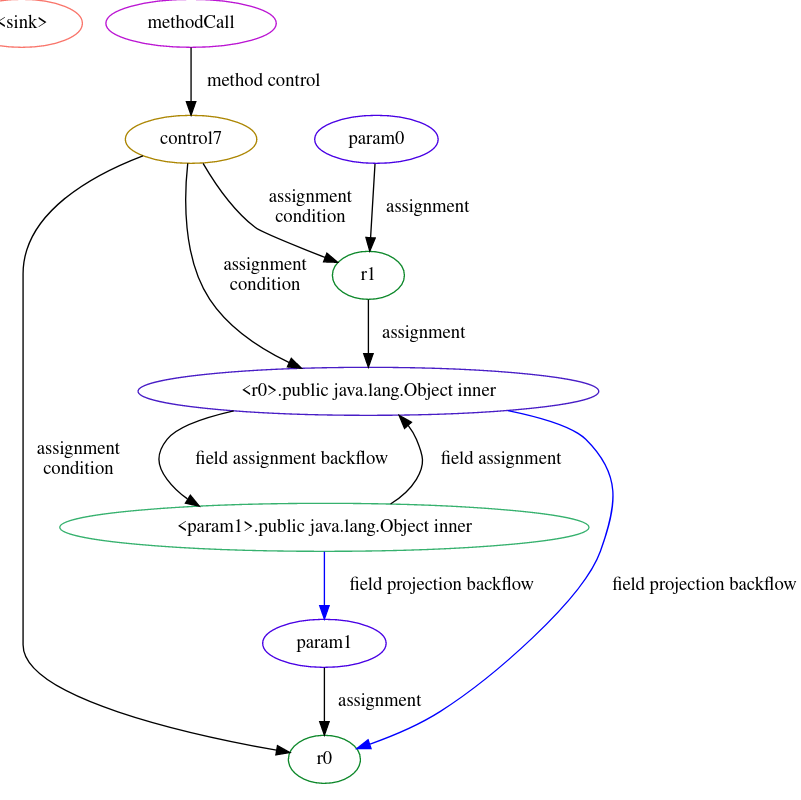
\includegraphics[scale=0.35]{screenshot20201231224543.png}
  \label{fig:param-to-param-lfg}
\end{figure}

Note the mutual flow between the nodes
\code{<r0>.public java.lang.Object.inner} and
\code{<param1>.public java.lang.Object.inner}.
Since \code{param1} is assigned into the local temporary \code{r0},
they point to the same value,
so their common field \code{inner} are located at the same address,
hence flow to one node always flows to the other.

\subsubsection{Control flow}
Branches and loops involve more \fnname{Control} nodes in the \ac{LFG}.

Consider the loop tests in Listing~\ref{lst:loop-tests}.
The \code{loopDec} method effectively copies \code{i} to \code{a},
leaking the parameter to return value by control flow.
The \fnname{Control} from branching by \code{i} covers the assignment of \code{a},
allowing it to reach the return path.
Similarly, the \code{whileCall} method uses
the return proxy node of \code{supplier.getAsBoolean()} to branch,
leaking any possible returned flow from \code{getAsBoolean()} to its own return path.

\IncludeCodePart{lst:loop-tests}
{../core/src/test/java/io/github/sof3/enclavlow/cases/lfg/LoopCase.java}
{Loop test cases}
{16}{30}

The test results can be reproduced with the Gradle test task.
Consult the GitHub CI setup at \url{https://github.com/SOF3/enclavlow/actions}
for details on environment setup.
Other unit tests in the project are omitted in this report
as their functionalities are insignificant or already covered by the above cases.

\subsection{Performance}
To analyze the performance of \pname{} in real projects,
a test application is written to run the \pname{} gradle plugin with.
The source code is available under the \code{example/} directory on the GitHub repository.
The test application opens a UDP socket that listens for packets
and computes a 6-digit one-time-password from the packet data.

The application involves the 6 simple methods of its own,
as well as the following methods from Java standard library:

\begin{itemize}
  \item \code{DatagramPacket.getData()}
  \item \code{DatagramPacket.new(byte[], int)}
  \item \code{DatagramPacket.setData(byte[])}
  \item \code{DatagramSocket.bind(InetSocketAddress)}
  \item \code{DatagramSocket.isClosed()}
  \item \code{DatagramSocket.new()}
  \item \code{DatagramSocket.receive(DatagramPacket)}
  \item \code{DatagramSocket.send(DatagramPacket)}
  \item \code{InetSocketAddress.new(String, int)}
  \item \code{System.currentTimeMillis()}
\end{itemize}

Due to transitive method calls,
it is found that 1806 different methods were eventually included in the analysis
(including native and abstract methods, which are not handled correctly;
see section \ref{subsec:difficulties-and-limitations} for details).
A total of 86 seconds were spent for analysis on an Intel i7-10510U CPU (1.80GHz)
(number of cores does not matter since the program is largely single-threaded)
on Linux kernel 5.4.0-58-generic with Java profiler enabled.

Profiler result shows that, among the 56 seconds of CPU time used on running Java code
(the remaining is attributed to JVM native operations),
76.8\% time is spent on \code{soot.SootResolver.resolveClass},
which is the part where Soot compiles the Java bytecode into its own representation.
Only 18.7\% time was actually spent on code from this project,
i.e. the part performing flow analysis.

Since Soot is not thread-safe due to its unfortunately aggressive use of static variables,
it is not possible to improve performance using parallelism.
Major change on the Soot framework or \ac{JVM} forking is necessary
for performance improvement.

Soot issues aside,
a large amount of CPU time is spent
on repacking the \ac{LFG} due to node removal.
A more efficient graph representation structure (such as layered views)
may be helpful in improving performance in this part.

A full profiler report can be found at \code{docs/profiler-results.jfr} on the GitHub repository.
Figures \ref{fig:flame-graph-full} and \ref{fig:flame-graph-analysis}
show the flame graph of profiler samples.

\begin{figure}
  \caption{Profiler flame graph (full)}
  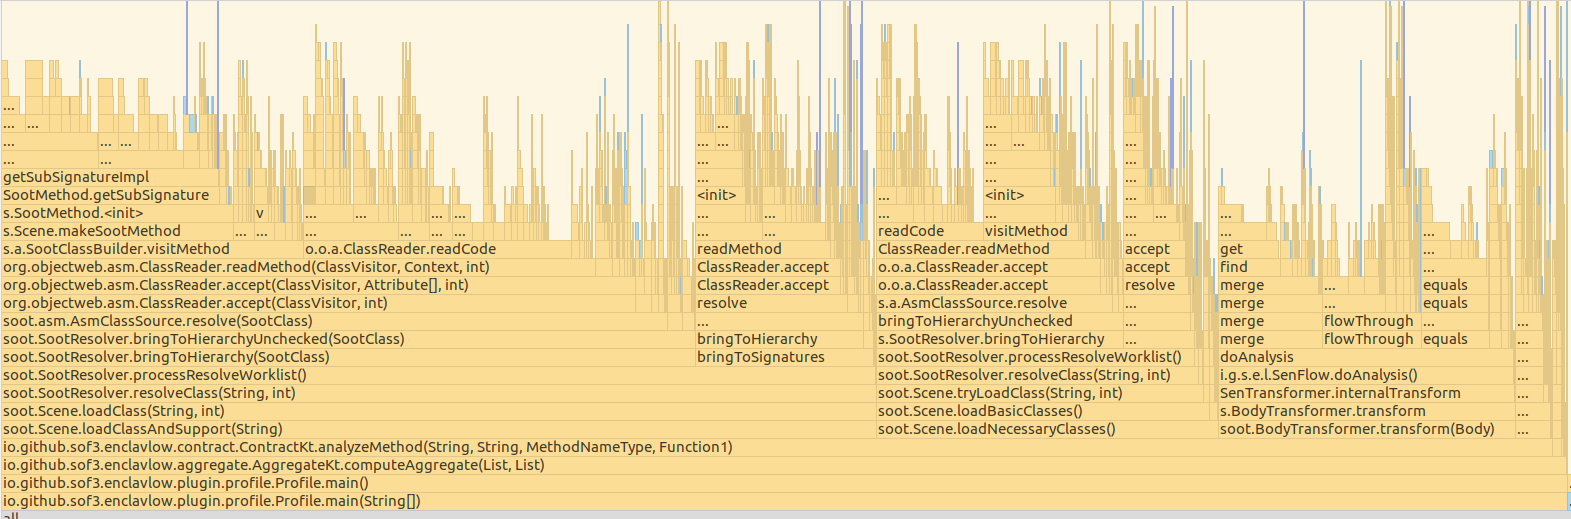
\includegraphics[scale=0.33]{screenshot20201231183130.png}
  \label{fig:flame-graph-full}
\end{figure}

\begin{figure}
  \caption{Profiler flame graph (analysis only)}
  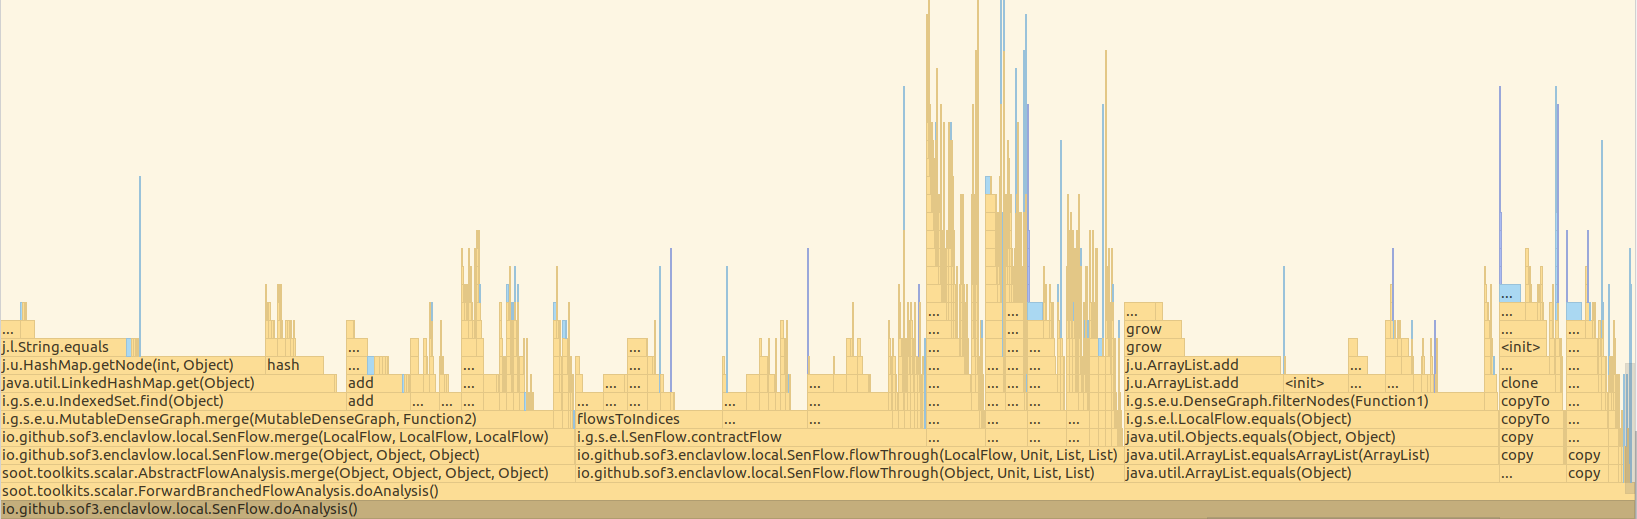
\includegraphics[scale=0.3]{screenshot20201231183716.png}
  \label{fig:flame-graph-analysis}
\end{figure}
